\section*{Exercise 2}
\textbf{Use complete graphs and counting arguments to show the following.}
\begin{enumerate}[a)]
    \item We will prove the claim using complete graphs. Let $n$ be the number of vertices in a graph $G$. Then, $\binom{n}{2}$ is the cardinality of the edge set of $G$, hence $|E(G)| = \frac{n(n-1)}{2}$. \\
    \linebreak 
    Take a complete graph on $n$ vertices $\mathcal{K}_n$. To make the explanation more apparent we will use an example graph below with $n = 5$ and $k = 3$, note that the meaning of all of the components inside the equation can be generalized.
\begin{enumerate}
    \item $\binom{n}{2}$ is just the number of edges in a complete graph, in our case it amounts to 20.
        \begin{center}
    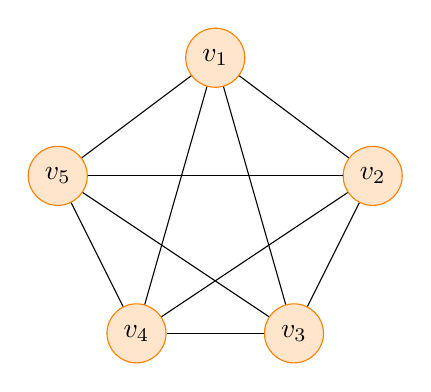
\begin{tikzpicture}
    \tikzset{% This is the style settings for nodes
    dep/.style={circle,minimum size=0.75cm,fill=orange!20,draw=orange},
    c1/.style={-},
    c2/.style={dotted, red, line width=2},
    %c2/.style={orange}, 
    }
    % Nodes
    \node[dep] (n1) at (3,3) {$v_1$};
    \node[dep] (n2) at (5,1.5) {$v_2$};
    \node[dep] (n3) at (4, -0.5) {$v_3$}; 
    \node[dep] (n4) at (2, -0.5) {$v_4$};
    \node[dep] (n5) at (1, 1.5) {$v_5$};

    %Edges
    \draw[c1] (n1) edge node[above] {} (n2);
    \draw[c1] (n1) edge node[above] {} (n3);
    \draw[c1] (n1) edge node[above] {} (n4);
    \draw[c1] (n1) edge node[above] {} (n5);
    \draw[c1] (n2) edge node[above] {} (n3);
    \draw[c1] (n2) edge node[above] {} (n4);
    \draw[c1] (n2) edge node[above] {} (n5);
    \draw[c1] (n3) edge node[above] {} (n4);
    \draw[c1] (n3) edge node[above] {} (n5);
    \draw[c1] (n4) edge node[above] {} (n5);

\end{tikzpicture}   
\end{center}
    \item $\binom{k}{2}$ is the size of a clique chosen inside the graph of size $k$. We know that this clique must exist for any choice of $k$ vertices, as the graph would otherwise not be complete. This accounts for all of the edges contained inside the clique and nothing more. We will call this subgraph $H$. In our specific case the size of the clique is 3 (in red below).
        \begin{center}
    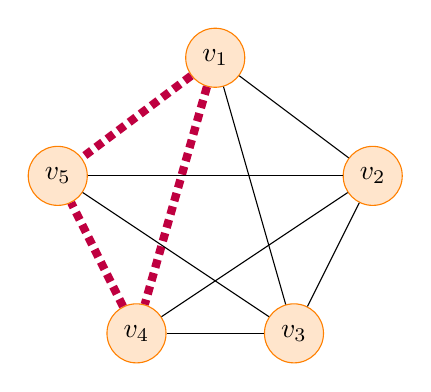
\begin{tikzpicture}
    \tikzset{% This is the style settings for nodes
    dep/.style={circle,minimum size=0.75cm,fill=orange!20,draw=orange},
    c1/.style={-},
    c2/.style={dotted, purple, line width=3},
    %c2/.style={orange}, 
    }
    % Nodes
    \node[dep] (n1) at (3,3) {$v_1$};
    \node[dep] (n2) at (5,1.5) {$v_2$};
    \node[dep] (n3) at (4, -0.5) {$v_3$}; 
    \node[dep] (n4) at (2, -0.5) {$v_4$};
    \node[dep] (n5) at (1, 1.5) {$v_5$};

    %Edges
    \draw[c1] (n1) edge node[above] {} (n2);
    \draw[c1] (n1) edge node[above] {} (n3);
    \draw[c2] (n1) edge node[above] {} (n4);
    \draw[c2] (n1) edge node[above] {} (n5);
    \draw[c1] (n2) edge node[above] {} (n3);
    \draw[c1] (n2) edge node[above] {} (n4);
    \draw[c1] (n2) edge node[above] {} (n5);
    \draw[c1] (n3) edge node[above] {} (n4);
    \draw[c1] (n3) edge node[above] {} (n5);
    \draw[c2] (n4) edge node[above] {} (n5);

\end{tikzpicture}   
\end{center}
    \item $k(n - k)$ is the amount of edges that link any vertex inside $H$ with any vertex outside of $H$, we will call this second subgraph $H'$. In our specific case the number of edges connecting $H$ and $H'$ is 6 (in green below).
    \begin{center}
    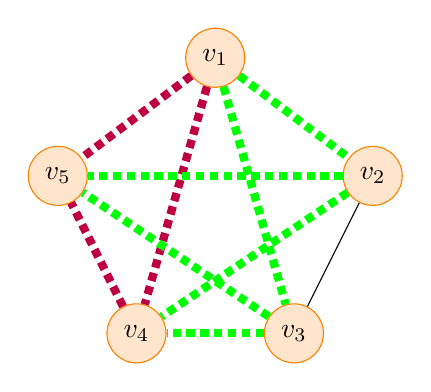
\begin{tikzpicture}
    \tikzset{% This is the style settings for nodes
    dep/.style={circle,minimum size=0.75cm,fill=orange!20,draw=orange},
    c1/.style={-},
    c2/.style={dotted, purple, line width=3},
    c3/.style={dotted, green, line width=3},
    %c2/.style={orange}, 
    }
    % Nodes
    \node[dep] (n1) at (3,3) {$v_1$};
    \node[dep] (n2) at (5,1.5) {$v_2$};
    \node[dep] (n3) at (4, -0.5) {$v_3$}; 
    \node[dep] (n4) at (2, -0.5) {$v_4$};
    \node[dep] (n5) at (1, 1.5) {$v_5$};

    %Edges
    \draw[c3] (n1) edge node[above] {} (n2);
    \draw[c3] (n1) edge node[above] {} (n3);
    \draw[c2] (n1) edge node[above] {} (n4);
    \draw[c2] (n1) edge node[above] {} (n5);
    \draw[c1] (n2) edge node[above] {} (n3);
    \draw[c3] (n2) edge node[above] {} (n4);
    \draw[c3] (n2) edge node[above] {} (n5);
    \draw[c3] (n3) edge node[above] {} (n4);
    \draw[c3] (n3) edge node[above] {} (n5);
    \draw[c2] (n4) edge node[above] {} (n5);

\end{tikzpicture}   
\end{center}
    \item $\binom{n - k}{2}$ is the amount of edges that connect all of the vertices that are inside $H'$, thus outside of our clique. In our specific case we have just the one show in blue below.
    \begin{center}
    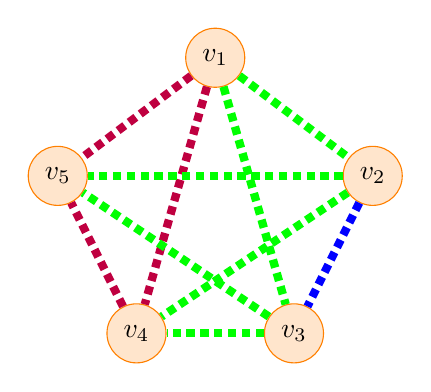
\begin{tikzpicture}
    \tikzset{% This is the style settings for nodes
    dep/.style={circle,minimum size=0.75cm,fill=orange!20,draw=orange},
    c1/.style={-},
    c2/.style={dotted, purple, line width=3},
    c3/.style={dotted, green, line width=3},
    c4/.style={dotted, blue, line width=3},
    %c2/.style={orange}, 
    }
    % Nodes
    \node[dep] (n1) at (3,3) {$v_1$};
    \node[dep] (n2) at (5,1.5) {$v_2$};
    \node[dep] (n3) at (4, -0.5) {$v_3$}; 
    \node[dep] (n4) at (2, -0.5) {$v_4$};
    \node[dep] (n5) at (1, 1.5) {$v_5$};

    %Edges
    \draw[c3] (n1) edge node[above] {} (n2);
    \draw[c3] (n1) edge node[above] {} (n3);
    \draw[c2] (n1) edge node[above] {} (n4);
    \draw[c2] (n1) edge node[above] {} (n5);
    \draw[c4] (n2) edge node[above] {} (n3);
    \draw[c3] (n2) edge node[above] {} (n4);
    \draw[c3] (n2) edge node[above] {} (n5);
    \draw[c3] (n3) edge node[above] {} (n4);
    \draw[c3] (n3) edge node[above] {} (n5);
    \draw[c2] (n4) edge node[above] {} (n5);

\end{tikzpicture}   
\end{center}
\end{enumerate}
All in all we are saying the following, if we consider a complete graph:
\begin{align*}
    \text{Total number of edges} &= \text{Edges inside a clique of size $k$} \\ &+ \text{Number of edges connecting the clique to the rest of the graph} \\ &+ \text{Edges that connect the nodes that are not in the clique}
\end{align*}
We can prove the above also by doing some computations by hand, the process is the following 
$\binom{n}{2} = \binom{k}{2} + k(n-k) + \binom{n-k}{2} \text{ for } 0 \leq k \leq n $ \\
\linebreak 
We know that \begin{equation}\binom{n}{k} = \frac{n!}{k!(n-k)!}\end{equation} \\ 
Therefore, \\
\linebreak 
\begin{equation}
    \binom{n}{2} = \frac{n!}{2!(n-2)!} = \frac{n!}{2(n-2)}
\end{equation}
\begin{equation}
    \binom{k}{2} = \frac{k!}{2!(k-2)!} = \frac{k!}{2(k-2)}
\end{equation}
\begin{equation}
    \binom{n-k}{2} = \frac{(n-k)!}{2!(n-k-2)!} = \frac{(n-k)!}{2(n-k-2)!}
\end{equation}
Hence, 
\begin{align}
\notag
    \frac{n!}{2(n-2)!} &= \frac{k!}{2(k-2)!} + k(n-k) + \frac{(n-k)!}{2(n-k-2)!} \\
    \notag
    \frac{n(n-1)}{2} &= \frac{k(k-1)}{2} + k(n-k) + \frac{(n-k)(n-k-1)}{2} \\
    \notag
    n(n-1) &= k(k-1) + 2(k(n-k)) + (n-k)(n-k-1) \\
    \notag
    n^2 - n &= k^2 - k + 2nk - 2k^2 + n^2 - nk - n - nk + k^2 + k \\
    n^2 - n &= n^2 - n \hspace{7cm} \square
\end{align}
    
    \item If $\Sigma^k_{i=1}n_1 = n \text{ for } 
 n_1, ..., n_k \in \mathbb{N}_0, \text{ then } \Sigma^k_{i=1} \binom{n_i}{2} \leq \binom{n}{2}$ \\
 \linebreak 
 Let's consider the following graph:
 \begin{center}
    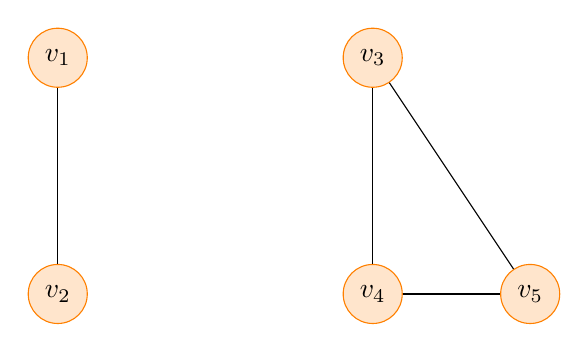
\begin{tikzpicture}
    \tikzset{% This is the style settings for nodes
    dep/.style={circle,minimum size=0.75cm,fill=orange!20,draw=orange},
    c1/.style={-},
    }
    % Nodes
    \node[dep] (n1) at (-4,3) {$v_1$};
    \node[dep] (n2) at (-4,0) {$v_2$};
    \node[dep] (n3) at (0, 3) {$v_3$}; 
    \node[dep] (n4) at (0, 0) {$v_4$};
    \node[dep] (n5) at (2, 0) {$v_5$};

    %Edges
    \draw[c1] (n1) edge node[above] {} (n2);
    \draw[c1] (n3) edge node[above] {} (n4);
    \draw[c1] (n4) edge node[above] {} (n5);
    \draw[c1] (n3) edge node[above] {} (n5);
\end{tikzpicture}   
\end{center}
Each component is a complete graph of its own, if we consider the following:
\begin{equation*}
    \sum_{i = 1}^k{\binom{n_i}{2}} = \sum_{i = 1}^k{e(K_{n_i})} = e(G) \leq \binom{n}{2}
\end{equation*}
\end{enumerate}